% Options for packages loaded elsewhere
\PassOptionsToPackage{unicode}{hyperref}
\PassOptionsToPackage{hyphens}{url}
\PassOptionsToPackage{dvipsnames,svgnames,x11names}{xcolor}
%
\documentclass[
  letterpaper,
  DIV=11,
  numbers=noendperiod]{scrartcl}

\usepackage{amsmath,amssymb}
\usepackage{iftex}
\ifPDFTeX
  \usepackage[T1]{fontenc}
  \usepackage[utf8]{inputenc}
  \usepackage{textcomp} % provide euro and other symbols
\else % if luatex or xetex
  \usepackage{unicode-math}
  \defaultfontfeatures{Scale=MatchLowercase}
  \defaultfontfeatures[\rmfamily]{Ligatures=TeX,Scale=1}
\fi
\usepackage{lmodern}
\ifPDFTeX\else  
    % xetex/luatex font selection
\fi
% Use upquote if available, for straight quotes in verbatim environments
\IfFileExists{upquote.sty}{\usepackage{upquote}}{}
\IfFileExists{microtype.sty}{% use microtype if available
  \usepackage[]{microtype}
  \UseMicrotypeSet[protrusion]{basicmath} % disable protrusion for tt fonts
}{}
\makeatletter
\@ifundefined{KOMAClassName}{% if non-KOMA class
  \IfFileExists{parskip.sty}{%
    \usepackage{parskip}
  }{% else
    \setlength{\parindent}{0pt}
    \setlength{\parskip}{6pt plus 2pt minus 1pt}}
}{% if KOMA class
  \KOMAoptions{parskip=half}}
\makeatother
\usepackage{xcolor}
\setlength{\emergencystretch}{3em} % prevent overfull lines
\setcounter{secnumdepth}{5}
% Make \paragraph and \subparagraph free-standing
\makeatletter
\ifx\paragraph\undefined\else
  \let\oldparagraph\paragraph
  \renewcommand{\paragraph}{
    \@ifstar
      \xxxParagraphStar
      \xxxParagraphNoStar
  }
  \newcommand{\xxxParagraphStar}[1]{\oldparagraph*{#1}\mbox{}}
  \newcommand{\xxxParagraphNoStar}[1]{\oldparagraph{#1}\mbox{}}
\fi
\ifx\subparagraph\undefined\else
  \let\oldsubparagraph\subparagraph
  \renewcommand{\subparagraph}{
    \@ifstar
      \xxxSubParagraphStar
      \xxxSubParagraphNoStar
  }
  \newcommand{\xxxSubParagraphStar}[1]{\oldsubparagraph*{#1}\mbox{}}
  \newcommand{\xxxSubParagraphNoStar}[1]{\oldsubparagraph{#1}\mbox{}}
\fi
\makeatother

\usepackage{color}
\usepackage{fancyvrb}
\newcommand{\VerbBar}{|}
\newcommand{\VERB}{\Verb[commandchars=\\\{\}]}
\DefineVerbatimEnvironment{Highlighting}{Verbatim}{commandchars=\\\{\}}
% Add ',fontsize=\small' for more characters per line
\usepackage{framed}
\definecolor{shadecolor}{RGB}{241,243,245}
\newenvironment{Shaded}{\begin{snugshade}}{\end{snugshade}}
\newcommand{\AlertTok}[1]{\textcolor[rgb]{0.68,0.00,0.00}{#1}}
\newcommand{\AnnotationTok}[1]{\textcolor[rgb]{0.37,0.37,0.37}{#1}}
\newcommand{\AttributeTok}[1]{\textcolor[rgb]{0.40,0.45,0.13}{#1}}
\newcommand{\BaseNTok}[1]{\textcolor[rgb]{0.68,0.00,0.00}{#1}}
\newcommand{\BuiltInTok}[1]{\textcolor[rgb]{0.00,0.23,0.31}{#1}}
\newcommand{\CharTok}[1]{\textcolor[rgb]{0.13,0.47,0.30}{#1}}
\newcommand{\CommentTok}[1]{\textcolor[rgb]{0.37,0.37,0.37}{#1}}
\newcommand{\CommentVarTok}[1]{\textcolor[rgb]{0.37,0.37,0.37}{\textit{#1}}}
\newcommand{\ConstantTok}[1]{\textcolor[rgb]{0.56,0.35,0.01}{#1}}
\newcommand{\ControlFlowTok}[1]{\textcolor[rgb]{0.00,0.23,0.31}{\textbf{#1}}}
\newcommand{\DataTypeTok}[1]{\textcolor[rgb]{0.68,0.00,0.00}{#1}}
\newcommand{\DecValTok}[1]{\textcolor[rgb]{0.68,0.00,0.00}{#1}}
\newcommand{\DocumentationTok}[1]{\textcolor[rgb]{0.37,0.37,0.37}{\textit{#1}}}
\newcommand{\ErrorTok}[1]{\textcolor[rgb]{0.68,0.00,0.00}{#1}}
\newcommand{\ExtensionTok}[1]{\textcolor[rgb]{0.00,0.23,0.31}{#1}}
\newcommand{\FloatTok}[1]{\textcolor[rgb]{0.68,0.00,0.00}{#1}}
\newcommand{\FunctionTok}[1]{\textcolor[rgb]{0.28,0.35,0.67}{#1}}
\newcommand{\ImportTok}[1]{\textcolor[rgb]{0.00,0.46,0.62}{#1}}
\newcommand{\InformationTok}[1]{\textcolor[rgb]{0.37,0.37,0.37}{#1}}
\newcommand{\KeywordTok}[1]{\textcolor[rgb]{0.00,0.23,0.31}{\textbf{#1}}}
\newcommand{\NormalTok}[1]{\textcolor[rgb]{0.00,0.23,0.31}{#1}}
\newcommand{\OperatorTok}[1]{\textcolor[rgb]{0.37,0.37,0.37}{#1}}
\newcommand{\OtherTok}[1]{\textcolor[rgb]{0.00,0.23,0.31}{#1}}
\newcommand{\PreprocessorTok}[1]{\textcolor[rgb]{0.68,0.00,0.00}{#1}}
\newcommand{\RegionMarkerTok}[1]{\textcolor[rgb]{0.00,0.23,0.31}{#1}}
\newcommand{\SpecialCharTok}[1]{\textcolor[rgb]{0.37,0.37,0.37}{#1}}
\newcommand{\SpecialStringTok}[1]{\textcolor[rgb]{0.13,0.47,0.30}{#1}}
\newcommand{\StringTok}[1]{\textcolor[rgb]{0.13,0.47,0.30}{#1}}
\newcommand{\VariableTok}[1]{\textcolor[rgb]{0.07,0.07,0.07}{#1}}
\newcommand{\VerbatimStringTok}[1]{\textcolor[rgb]{0.13,0.47,0.30}{#1}}
\newcommand{\WarningTok}[1]{\textcolor[rgb]{0.37,0.37,0.37}{\textit{#1}}}

\providecommand{\tightlist}{%
  \setlength{\itemsep}{0pt}\setlength{\parskip}{0pt}}\usepackage{longtable,booktabs,array}
\usepackage{calc} % for calculating minipage widths
% Correct order of tables after \paragraph or \subparagraph
\usepackage{etoolbox}
\makeatletter
\patchcmd\longtable{\par}{\if@noskipsec\mbox{}\fi\par}{}{}
\makeatother
% Allow footnotes in longtable head/foot
\IfFileExists{footnotehyper.sty}{\usepackage{footnotehyper}}{\usepackage{footnote}}
\makesavenoteenv{longtable}
\usepackage{graphicx}
\makeatletter
\def\maxwidth{\ifdim\Gin@nat@width>\linewidth\linewidth\else\Gin@nat@width\fi}
\def\maxheight{\ifdim\Gin@nat@height>\textheight\textheight\else\Gin@nat@height\fi}
\makeatother
% Scale images if necessary, so that they will not overflow the page
% margins by default, and it is still possible to overwrite the defaults
% using explicit options in \includegraphics[width, height, ...]{}
\setkeys{Gin}{width=\maxwidth,height=\maxheight,keepaspectratio}
% Set default figure placement to htbp
\makeatletter
\def\fps@figure{htbp}
\makeatother

\KOMAoption{captions}{tableheading}
\makeatletter
\@ifpackageloaded{tcolorbox}{}{\usepackage[skins,breakable]{tcolorbox}}
\@ifpackageloaded{fontawesome5}{}{\usepackage{fontawesome5}}
\definecolor{quarto-callout-color}{HTML}{909090}
\definecolor{quarto-callout-note-color}{HTML}{0758E5}
\definecolor{quarto-callout-important-color}{HTML}{CC1914}
\definecolor{quarto-callout-warning-color}{HTML}{EB9113}
\definecolor{quarto-callout-tip-color}{HTML}{00A047}
\definecolor{quarto-callout-caution-color}{HTML}{FC5300}
\definecolor{quarto-callout-color-frame}{HTML}{acacac}
\definecolor{quarto-callout-note-color-frame}{HTML}{4582ec}
\definecolor{quarto-callout-important-color-frame}{HTML}{d9534f}
\definecolor{quarto-callout-warning-color-frame}{HTML}{f0ad4e}
\definecolor{quarto-callout-tip-color-frame}{HTML}{02b875}
\definecolor{quarto-callout-caution-color-frame}{HTML}{fd7e14}
\makeatother
\makeatletter
\@ifpackageloaded{caption}{}{\usepackage{caption}}
\AtBeginDocument{%
\ifdefined\contentsname
  \renewcommand*\contentsname{Table of contents}
\else
  \newcommand\contentsname{Table of contents}
\fi
\ifdefined\listfigurename
  \renewcommand*\listfigurename{List of Figures}
\else
  \newcommand\listfigurename{List of Figures}
\fi
\ifdefined\listtablename
  \renewcommand*\listtablename{List of Tables}
\else
  \newcommand\listtablename{List of Tables}
\fi
\ifdefined\figurename
  \renewcommand*\figurename{Figure}
\else
  \newcommand\figurename{Figure}
\fi
\ifdefined\tablename
  \renewcommand*\tablename{Table}
\else
  \newcommand\tablename{Table}
\fi
}
\@ifpackageloaded{float}{}{\usepackage{float}}
\floatstyle{ruled}
\@ifundefined{c@chapter}{\newfloat{codelisting}{h}{lop}}{\newfloat{codelisting}{h}{lop}[chapter]}
\floatname{codelisting}{Listing}
\newcommand*\listoflistings{\listof{codelisting}{List of Listings}}
\makeatother
\makeatletter
\makeatother
\makeatletter
\@ifpackageloaded{caption}{}{\usepackage{caption}}
\@ifpackageloaded{subcaption}{}{\usepackage{subcaption}}
\makeatother

\ifLuaTeX
  \usepackage{selnolig}  % disable illegal ligatures
\fi
\usepackage{bookmark}

\IfFileExists{xurl.sty}{\usepackage{xurl}}{} % add URL line breaks if available
\urlstyle{same} % disable monospaced font for URLs
\hypersetup{
  pdftitle={Introducción a R para investigación y ciencia de datos},
  pdfauthor={Gema Fernández-Avilés Calderón},
  colorlinks=true,
  linkcolor={blue},
  filecolor={Maroon},
  citecolor={Blue},
  urlcolor={Blue},
  pdfcreator={LaTeX via pandoc}}


\title{Introducción a R para investigación y ciencia de datos}
\usepackage{etoolbox}
\makeatletter
\providecommand{\subtitle}[1]{% add subtitle to \maketitle
  \apptocmd{\@title}{\par {\large #1 \par}}{}{}
}
\makeatother
\subtitle{Pre-curso}
\author{Gema Fernández-Avilés Calderón}
\date{2024-12-03}

\begin{document}
\maketitle

\renewcommand*\contentsname{Table of contents}
{
\hypersetup{linkcolor=}
\setcounter{tocdepth}{3}
\tableofcontents
}

\section{Pre-curso ⏰}\label{pre-curso}


\includegraphics{img/00-Rlearners.png}

Bienvenidos al curso \textbf{Introducción a R para investigación y
ciencia de datos}. Es aconsejable que tengamos preparados nuestros
ordenadores antes de comenzar el curso. Para ello, por favor, lee y
realiza las siguientes acciones:

\subsection{Descarga e instala R en tu
PC}\label{descarga-e-instala-r-en-tu-pc}

Ve a la página \url{https://cloud.r-project.org/} y elige la opción
conveniende en función de tu sistema operativo: Linux (Debian,
Fedora/Redhat, Ubuntu), macOS o Windows. Al finalizar, verás el icono de
\textbf{R} como acceso directo en tu estcritorio.

\subsection{Descarga e instala
RStudio}\label{descarga-e-instala-rstudio}

Ve a la página \url{https://posit.co/download/rstudio-desktop/} y
descarga e instala Rstudio. En función de las características de tu PC,
la propia aplicación suele recomendarte la versión adecuada.

Puede ocurrir que no se cree el acceso directo de RStudio en tu
escritorio. Si quieres poner un accedo directo a RStudio, en el buscador
del ordenador (si tienes Windows se encuentra en la esquina inferior
izquierda) escribe RStudio y ve a la carpeta que contiene la ubicación
del programa. Desde allí, pinchando con el botón derecho del ratón sobre
el icono de RStudio puedes crear un acceso directo a RStudio en el
Escritorio.

Al final los dos primeros pasos tendrás en tu escritorio estos dos
iconos como accesos directos:

\begin{figure}[H]

{\centering 
\includegraphics[width=0.3\textwidth,height=\textheight]{img/r-rstudio-icons.png}

}

\caption{Icono de R (izquierda) y RStudio (derecha)}

\end{figure}%

\subsection{Abre R console e instala los paquetes
siguientes.}\label{abre-r-console-e-instala-los-paquetes-siguientes.}

De los iconos anteriores, abre el icono de \textbf{R}.

\begin{figure}[H]

{\centering 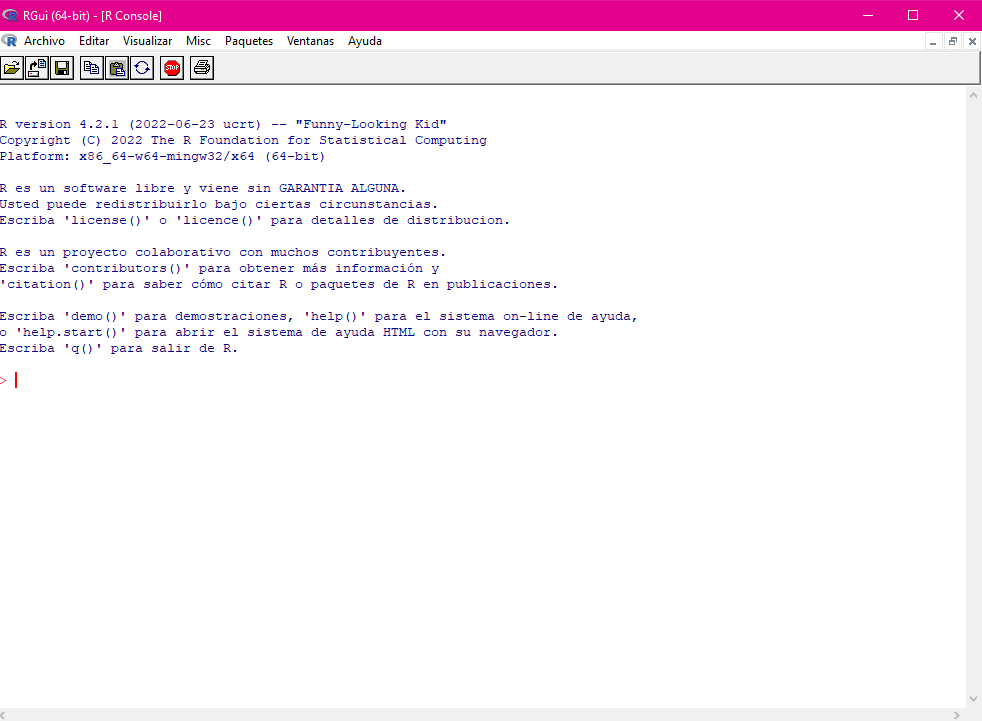
\includegraphics[width=0.3\textwidth,height=\textheight]{img/r-console.png}

}

\caption{\textbf{Consola de R.}}

\end{figure}%

\subsection{Descarga e instalación de
paquetes}\label{descarga-e-instalaciuxf3n-de-paquetes}

En la consola de \textbf{R}, copia y pega el siguiente código para
instalar estos paquetes de paquetes:

\begin{Shaded}
\begin{Highlighting}[]
\FunctionTok{install.packages}\NormalTok{(}\StringTok{\textquotesingle{}rmarkdown\textquotesingle{}}\NormalTok{) }
\FunctionTok{install.packages}\NormalTok{(}\StringTok{\textquotesingle{}tidyverse\textquotesingle{}}\NormalTok{)}
\FunctionTok{install.packages}\NormalTok{(}\StringTok{\textquotesingle{}rlang\textquotesingle{}}\NormalTok{)}
\FunctionTok{install.packages}\NormalTok{(}\StringTok{\textquotesingle{}leaflet\textquotesingle{}}\NormalTok{) }
\FunctionTok{install.packages}\NormalTok{(}\StringTok{\textquotesingle{}leaflet.extras\textquotesingle{}}\NormalTok{) }
\FunctionTok{install.packages}\NormalTok{(}\StringTok{\textquotesingle{}leaflet.providers\textquotesingle{}}\NormalTok{) }
\FunctionTok{install.packages}\NormalTok{(}\StringTok{\textquotesingle{}plotly\textquotesingle{}}\NormalTok{)}
\FunctionTok{install.packages}\NormalTok{(}\StringTok{\textquotesingle{}rvest\textquotesingle{}}\NormalTok{)}
\FunctionTok{install.packages}\NormalTok{(}\StringTok{"palmerpenguins"}\NormalTok{)}
\FunctionTok{install.packages}\NormalTok{(}\StringTok{\textquotesingle{}gapminder\textquotesingle{}}\NormalTok{)}
\FunctionTok{install.packages}\NormalTok{(}\StringTok{\textquotesingle{}HistData\textquotesingle{}}\NormalTok{)}
\FunctionTok{install.packages}\NormalTok{(}\StringTok{\textquotesingle{}skimr\textquotesingle{}}\NormalTok{) }
\FunctionTok{install.packages}\NormalTok{(}\StringTok{\textquotesingle{}tseries\textquotesingle{}}\NormalTok{) }
\FunctionTok{install.packages}\NormalTok{(}\StringTok{\textquotesingle{}scales\textquotesingle{}}\NormalTok{) }
\FunctionTok{install.packages}\NormalTok{(}\StringTok{\textquotesingle{}kableExtra\textquotesingle{}}\NormalTok{) }
\FunctionTok{install.packages}\NormalTok{(}\StringTok{\textquotesingle{}knitr\textquotesingle{}}\NormalTok{) }
\FunctionTok{install.packages}\NormalTok{(}\StringTok{\textquotesingle{}learnr\textquotesingle{}}\NormalTok{)}
\FunctionTok{install.packages}\NormalTok{(}\StringTok{"remotes"}\NormalTok{)}
\NormalTok{remotes}\SpecialCharTok{::}\FunctionTok{install\_github}\NormalTok{(}\StringTok{"rstudio/gradethis"}\NormalTok{)}
\FunctionTok{install.packages}\NormalTok{(}\StringTok{\textquotesingle{}rio\textquotesingle{}}\NormalTok{)}
\FunctionTok{install.packages}\NormalTok{(}\StringTok{\textquotesingle{}readxl\textquotesingle{}}\NormalTok{)}
\FunctionTok{install.packages}\NormalTok{(}\StringTok{\textquotesingle{}fontawesome\textquotesingle{}}\NormalTok{)}
\FunctionTok{install.packages}\NormalTok{(}\StringTok{"devtools"}\NormalTok{)}
\NormalTok{devtools}\SpecialCharTok{::}\FunctionTok{install\_github}\NormalTok{(}\StringTok{"hadley/emo"}\NormalTok{)}
\end{Highlighting}
\end{Shaded}

\subsubsection{OPCIONAL: LATEX Y PDF}\label{opcional-latex-y-pdf}

\begin{itemize}
\tightlist
\item
  Opción (1): Instalar el paquete \{tinytex\}
\end{itemize}

\begin{Shaded}
\begin{Highlighting}[]
\FunctionTok{install.packages}\NormalTok{(}\StringTok{\textquotesingle{}tinytex\textquotesingle{}}\NormalTok{)}
\NormalTok{tinytex}\SpecialCharTok{::}\FunctionTok{install\_tinytex}\NormalTok{()}
\end{Highlighting}
\end{Shaded}

Una vez instalado, para comprobar su correcta instalación, ejecutar el
siguiente código R (copia y pega) en la consola:

\begin{Shaded}
\begin{Highlighting}[]
\FunctionTok{writeLines}\NormalTok{(}\FunctionTok{c}\NormalTok{(}
  \StringTok{\textquotesingle{}}\SpecialCharTok{\textbackslash{}\textbackslash{}}\StringTok{documentclass\{article\}\textquotesingle{}}\NormalTok{,}
  \StringTok{\textquotesingle{}}\SpecialCharTok{\textbackslash{}\textbackslash{}}\StringTok{begin\{document\}\textquotesingle{}}\NormalTok{, }\StringTok{\textquotesingle{}Hello world!\textquotesingle{}}\NormalTok{, }\StringTok{\textquotesingle{}}\SpecialCharTok{\textbackslash{}\textbackslash{}}\StringTok{end\{document\}\textquotesingle{}}
\NormalTok{), }\StringTok{\textquotesingle{}test.tex\textquotesingle{}}\NormalTok{)}
\NormalTok{tinytex}\SpecialCharTok{::}\FunctionTok{pdflatex}\NormalTok{(}\StringTok{\textquotesingle{}test.tex\textquotesingle{}}\NormalTok{)}
\end{Highlighting}
\end{Shaded}

\begin{verbatim}
[1] "test.pdf"
\end{verbatim}

El resultado es un archivo llamado ``test.pdf''.

\subsection{Índice del curso}\label{uxedndice-del-curso}

\begin{enumerate}
\def\labelenumi{\arabic{enumi}.}
\setcounter{enumi}{-1}
\item
  Presentación
\item
  Hola R.
\item
  \emph{Toolkit} del curso: RStduio, Quarto y Github.
\item
  Estructuras de datos en R.
\item
  Importación y exportación de datos.
\item
  Visualización de datos con \{ggplot2\}.
\item
  Manipulación de datos con \{tidyverse\}
\end{enumerate}


\includegraphics{img/icons8-code-R-64.png}

\begin{tcolorbox}[enhanced jigsaw, left=2mm, bottomrule=.15mm, coltitle=black, opacitybacktitle=0.6, colbacktitle=quarto-callout-note-color!10!white, rightrule=.15mm, opacityback=0, leftrule=.75mm, arc=.35mm, colback=white, colframe=quarto-callout-note-color-frame, breakable, titlerule=0mm, toptitle=1mm, bottomtitle=1mm, toprule=.15mm, title=\textcolor{quarto-callout-note-color}{\faInfo}\hspace{0.5em}{Nuestra filosofía: 📖 \emph{learning by doing}}]

\begin{itemize}
\item
  Recuerda que los ordenadores actualmente no son inteligentes.
\item
  Filosofía: \texttt{copy,\ paste,\ and\ tweak}.
\item
  La mejor forma de aprender código es haciéndolo.
\item
  La práctica es la clave.
\end{itemize}

\end{tcolorbox}

\textbf{Lo que NO aprenderás:}

\begin{itemize}
\tightlist
\item
  Programación en R.
\item
  Escritura en Latex.
\item
  Contenidos teóricos de ciencia de datos.
\end{itemize}

\begin{tcolorbox}[enhanced jigsaw, left=2mm, bottomrule=.15mm, coltitle=black, opacitybacktitle=0.6, colbacktitle=quarto-callout-tip-color!10!white, rightrule=.15mm, opacityback=0, leftrule=.75mm, arc=.35mm, colback=white, colframe=quarto-callout-tip-color-frame, breakable, titlerule=0mm, toptitle=1mm, bottomtitle=1mm, toprule=.15mm, title=\textcolor{quarto-callout-tip-color}{\faLightbulb}\hspace{0.5em}{Tip}]

Si tienes alguna duda, no dudes en escribirme a: 📮 gema.faviles@uclm.es

\end{tcolorbox}




\end{document}
